\documentclass{VUMIFInfKursinis}
\usepackage{algorithmicx}
\usepackage{algorithm}
\usepackage{algpseudocode}
\usepackage{amsfonts}
\usepackage{amsmath}
\usepackage{bm}
\usepackage{color}
\usepackage{graphicx}
% \usepackage{hyperref}  % Nuorodų aktyvavimas
\usepackage{url}
\graphicspath{ {./fjos/} }
\usepackage{systeme}

% Titulinio aprašas
\university{Vilniaus universitetas}
\faculty{Matematikos ir informatikos fakultetas}
\department{PROGRAMŲ SISTEMŲ BAKALAURO STUDIJŲ PROGRAMA}
\papertype{Kursinis darbas}
\title{Objektų atpažinimas ir sekimas kompiuterinės tomografijos vaizduose}
\titleineng{Object detection and tracking in computed tomography}
\status{3 kurso Programų sistemų studentas}
\author{Paulius Milmantas}
\supervisor{Linas Petkevičius}
\date{Vilnius \\ \the\year}

% Nustatymai
% \setmainfont{Palemonas}   % Pakeisti teksto šriftą į Palemonas (turi būti įdiegtas sistemoje)
\bibliography{bibliografija}

\begin{document}
\maketitle

\sectionnonum{Įvadas}
Pastaraisiais metais į medicinos sritį labai sparčiai skverbiasi informacinės technologijos. Atliekant
įvairias diagnostikas ar tiriant ligas, vaistus yra pasitelkiama programinių sistemų pagalba. Tačiau
didžiąją radiologo darbo dalį sprendimus turi priimti jis pats be jokios programinės įrangos pagalbos,
nors dažniausiai yra apibrėžti tam tikri ligų aptikimų algorimtai, kaip vėžinių lastelių aptikimas,
lūžiai ir taip toliau. Mano darbo tikslas yra prisidėti prie programinės įrangos kūrimo radiologams
ir sukurti programą, kuri aptinka plaučius, kad vėliau tai galėtų būti panaudota tolimesnei
IT plėtrai medicinos srityje.
\par
Šiandien viena iš labiausiai perspektyvių sričių informacinių technologijų srityje yra giliojo mokymosi
metodai.
Jie padeda duomenyse aptikti sunkiai pastebimus dėsningumus ir nuspėti išeities rezultatus su tam tikra klaidos tikimybe.
Šiame darbe kalbėsiu vieną iš šių metodų: dirbtinius neuroninius tinklus.
Juos pasirinkau nes kompiuterinės tomografijos vaizdai turi labai daug informacijos ir juos apdoroti
naudojant logines taisykles yra per daug sunku. Tačiau net ir jiems ši užduotis yra per sudėtinga, jeigu
tiriamos yra įvairios mutacijos arba nedažnos ligos, nes su kiekvienu nauju nematytu ligos atveju,
yra reikalinga apmokyti modelį, o tai reikalauja daug duomenų.
\par
%https://medium.com/@chiragsehra42/decision-trees-explained-easily-28f23241248
Pasirinktam mano dirbtinių neuroninių tinklų metodui viena iš galimų alternatyvų yra "sprendimo medžiai".
Tai yra prižiūrimo mokymosi metodas skirtas duomenų klasifikacijai ir duomenų regresijai. Šis metodas
naudoja taisyklių rinkinį. Norint gauti mažą šio metodo paklaidą, turime aprašyti vis daugiau šių taisyklių.
Taisyklės paprastai būna aprašomos naudojant "if, else" aprašus.\cite{salt1} Mano nagrinėjamame atvejyje duomenys
yra labai dideli ir įvairūs, todėl aprašyti visas šias taisykles užtruktų neproporcingai daug laiko ir tam
tikrų radiologijos žinių.
\par
Pasiekti darbo rezultatai: sukurtas neuroninis tinklas ir parašyta programa, kuri aptinka plaučius kompiuterinės tomografijos
nuotrauka. Pasiektas 0.02 nuostolių funkcijos rezultatas, naudojant 298 nuotraukose, kurios buvo gautos taikant
įvairias modifikacijas pradinėms 50 nuotraukų. Šis darbas įrodo, jog pasiekti aušktą
objektų aptikimą kompiuterinės tomografijos nuotraukose, nereikia turėti daug duomenų ir daug
resursų. Tai įmanoma padaryti ir naudojant Google Cloud platformą.

\tableofcontents

\section{Dirbtinio neuroninio tinklo sudėtis}
\subsection{Bazinė struktūra}
Daugelį dirbtinių neuronų tinklų sudaro panašios struktūrinės dalys:
\begin{enumerate}
  \item Įvesties sluoksnis: tai dalis kuri priima įvestį ir perduoda kitiems sluoksniams.
  Šiame darbe yra naudojamos kompiuterinės tomografijos nuotraukos, kurios yra suvienodinamos
  į 300x300 dydį. Nuotraukose yra pašalinamas RGB kanalas, todėl kiekvieną pikselį nusako
  pilkos spalvos atspalvis, kuris yra intervale [0;1]. Vienai nuotraukai užkoduoti
  užtenka 90 000 taškų, todėl neuroninio tinklo įvesties sluoksnį sudaro 90 000 neuronų.
  \item Išvesties sluoksnis: tai dalis, kuri naudoja aktyvacijos funkciją, kuri grąžina galutinį tinklo rezultatą: tikimybių rinkinį,
  kuris parodo kokia tikimybė, kad objektas atitinka tam tikrą klasę. Dažniausiai kiek
  uždavinyje yra klasių, tiek ir yra neuronų išvesties sluoksnyje.
  \item Paslėptas sluoksnis: perduoda svorius iš praeito sluoksnio į sekantį. Prieš reikšmės perdavimą paslėptame
  sluoksnyje kiekvienas neuronas sudeda visų ankstesnio sluoksnio neuronų siunčiamas reikšmes. Šią sumą
  neuronai siunčia toliau, tačiau jų reikšmės yra pakeičiamos atsižvelgiant į svorius tarp neuronų jungčių ir
  tendenciškumo.
  \item Susijungimai, jų svoriai ir tendenciškumas: Šie du parametrai yra
  tinklo automatiškai sugeneruojami ir apmokant tinklą pagal
  duomenis, svoriai ir tendenciškumas
  yra automatiškai tinklo keičiami. Tendenciškumas apibrėžia kaip tinklo išvestis yra nutolusi
  nuo tikrosios reikšmės. Tarp
  kiekvieno neurono, kuris yra susijungęs tarpusavyje, turi savo jungtis, per
  kurias yra paduodamos reikšmės kitiems neuronams sekančiuose sluoksniuose.
  Kaip reikšmė kis keliaujant per jungtis, nusako svoriai tarp jungčių. Tinklui mokantis
  šie svoriai yra keičiami tol, kols tinklo išvestis priartėja tikro atsakymo. Svoriai
  nurodo koks stiprus yra ryšys tarp neuronų, taip nurodant, kaip tinklo reikšmės kinta pačiame tinkle.
  Jeigu tinklui yra paduodama reikšmė, o pirmasis tinklo neuronas, kuris priima reikšmę turi mažą
  svorį, tai reiškia, jog galutiniams rezultatui ši reikšmė neturi daug įtakos. Jeigu svoris yra
  didelis, tai duota reikšmė turi daug įtakos rezultatui. \cite{salt2} Tinkluose yra
  taip pat naudojamas tendenciškumas. Jis nusako kaip turi būti koreguojamos tinklo reikšmės.
  Jeigu aktyvacijos funkcija grąžina blogą reikšmę, galima keisti tendenciškumo kintamajį ir
  pakeisti galutinį rezultatą.
  \item Aktyvacijos funkcija: tai funkcija, kokia turi būti neurono išvestis. Kiekvienas neuronas
  susumuoja praeito sluoksnio neuronų išvestis ir šią suma praleidžia pro aktyvacijos funkciją.
  Aktyvacijos funkcijos reikšmė yra toliau paduodama kitiems neuronams (atsižvelgiant taip pat ir į
  jungčių svorius ir į tendenciškumą).
  \item Optimizatimo funkcija: optimizuoja tikslo funkciją. Tikslo funkcija yra taip pat vadinama nuostolių funkcija.
  Šios funkcijos pagrindinis tikslas yra keisti neuroninio tinklo reikšmes taip, kad tinklo išvestis būtų
  kuo artimesnė tikram rezultatui.
  \item Mokymosi taisyklė: apibrėžia, kaip tinkle keičiasi svoriai, kad tinklas išvestų norimus rezultatus.
  Taip pat galima nurodyti ir kaip keičiasi tendenciškumas, bei kada jį naudoti.
\end{enumerate}
% https://deepai.org/machine-learning-glossary-and-terms/weight-artificial-neural-network
\par
Turint šias bazines neuroninio tinklo dalis, galima jį pradėti mokyti. Paprastai mokymasis
yra skiriamas į dvi dalis: priekinę ir galinę sklaidą.
% Priekine sklaida
Kai tinklui yra paduodamos reikšmės, jos keliauja iš pradinio sluoksnio iki išvesties sluoksnio. Tai
yra priekinė sklaida.
% Atgaline sklaida
% (http://didattica.cs.unicam.it/lib/exe/fetch.php?media=didattica:magistrale:kebi:ay_1718:ke-11_neural_networks.pdf University of Applied Sciences Northwestern Switzerland)
Atgalinė sklaida vyksta, kai tinklas išveda rezultatą, patikrinama ar
rezultatas yra teisingas ir atitinkamai tinklas reaguoja į tai. Inicijuojant tinklą svoriai yra
nustatomi atsitiktinai. Kiekvienam duomenų rinkiniui yra stebima tinklo išvestis ir tikrinama kokia
ji turėtų būti. Padaryta klaida yra perduodama tinklui atgal, per praeitus sluoksnius, einant nuo
išvesties sluoksnio. Šiame žingsnyje yra naudojama optimizavimo funkcija. Ji parodo kokie turėtų būti
svorių ir tendenciškumo pokyčiai tinklai ir taip yra
keičiami tinklo svoriai ir tendenciškumas atsižvelgiant į padarytą klaidą. Kai klaidos
yra padaromos pakankamai mažos ir jos yra mažesnės už duotą ribinę reikšmę, yra laikoma, kad tinklas
baigė mokymosi procesą. \cite{salt3}

\subsection{GPU naudojimas}
\par
Šiame darbe bus naudojamas GPU, atliekant tinklo treniravimą. Tai yra spartesnis būdas už CPU
naudojimas, nes CPU turi kelis galingus branduolius, o GPU žymiai daugiau. Giliajame mokyme,
naudojami aritmetiniai veiksmai yra ganėtinai paprasti, todėl juos apdoroti gali ir CPU ir GPU.
Tačiau GPU turi daugiau branduolių, kas leidžia atlikti daugiau matematinių veiksmų paralizuotai,
negul CPU. Taip yra pasiekiamas didesnis treniravimo našumas.
\par
Didesniam treniravimo našumui pastebėti naudojant GPU, negu CPU, buvo atliktas paprastas bandymas:
naudojant Google tensorflow struktūrą, apmokame sistemą atpažinti kur yra žmogaus plaučiai kompiuterinės
tomografijos vaizduose su CPU ir GPU. Vidutiniškai apdoruojant 60 megabaitų duomenų, vienam ciklui
tinklas su CPU resursais užtrunka 6 sekundes, o naudojant GPU vidutiniškai vienas žingsnis užtrunka
0.3 sekundės.
\par
% https://www.tensorflow.org/install/gpu
Šiame darbe naudojamas Tensorflow karkasas naudoja NVIDIA CUDA sistemą. \cite{salt4}
% https://developer.nvidia.com/cuda-zone
CUDA yra paralelinio skaičiavimo platforma, naudojama su grafikos plokštėmis. \cite{salt5}
Ji kiekvieną skaičiavimą paleidžia ant atskiros gijos. Visi duomenys yra suskirstyti
į vienos, dviejų ir trijų dimensijų blokus. Kiekvienams blogas gali turėti virš 512
gijų. Visos gijos kurios operuoja viename bloke dalinasi bendra GPU atmintimi.
Jeigu norima optimizuoti programą ir paleisti jos skaičiavimus ant GPU, tada reikia
suskaičiuoti kiek vyks paralelinių operacijų ir kiek iš jų dalinsis bendra atmintimi.
Pagal apskaičiuotą kiekį nurodome kiek mes norime turėti blokų ir kiek kiekvienas blokas
turės atskirų gijų. Prieš kiekvieną operaciją, siekiant pasiekti optimalų našumą, jeigu
reikia įkeliame kintamuosiu į bendrą bloko atmintį. Po atliktų skaičiavimų išvestus
rezultatus turime iškelti iš bendros atminties.
\par
Tačiau GPU naudojimas nėra visur panaudojamas. GPU gerai atlieka slankaus kablelio
operacijas (FLOPs) ir atminties pralaidumu. Jeigu problema reikalauja nepastovios atminties,
jos sprendimo paleidimas ant GPU nebus efektyvus, nes nebus galima išnaudoti branduolių,
dėl kintančios atminties. Taip pat problemos sprendimas nebus efektyvus, jeigu
reikalaus nedaug aritmetiškai intensyvių operacijų.

\subsection{Aktyvacijos funkcijos}
\par
Aktyvacijos funkcijos yra būtinos neuroniniame tinkle, jeigu norime, kad tinklas
grąžintų netiesines reikšmes. T.y. kad nuo tinklui duodamų parametrų, tinklo išvestis
nepriklausytų tiesiogiai. \cite{salt18} Neuroninio tinklo tikslas yra rasti tam tikrą
koreliaciją tarp įvesties ir išvesties duomenų. Jeigu duomenys yra sudėtingų struktūrų,
tiesinis tinklas koreliacijos neras, tačiau jeigu yra naudojamos aktyvacijos funkcijos,
tinklas yra netiesinis, tada galima aptikti labiau kompleksyvią koreliaciją. \cite{salt18}

\subsubsection{Tiesinė aktyvacijos funkcija}
\[
R(x, a) = x \cdot a
\]
\par
Tiesinės aktyvacijos funkcijos mių diapazonas yra labai didelis ir nėra dvejetainis,
kaip dalis kitų funkcijų. Tačiau ši funkcija nėra plačiai naudojama, nes jos
išvestinė yra konstanta, kas reiškia jog gautas gradientas nepriklauso nuo ‘x’.
Taigi, jeigu spėjime yra klaida, vykdant atgalinę sklaidą mes reikšmę taisysime
konstanta, neatsižvelgiant į pačią klaidą. \cite{salt16}

\begin{figure}[ht]
  \centering
  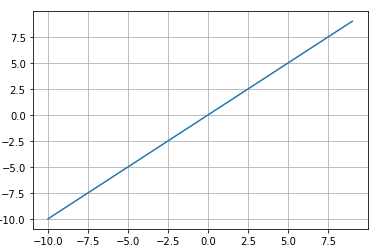
\includegraphics[width=6cm,height=6cm,keepaspectratio]{tiesine.png}
  \caption{Tiesinė lygtis}
  \label{fig:lygtis1}
\end{figure}

\subsubsection{ELU}
\[
  R(z) = \systeme*{z; z > 0, \alpha \cdot (e^z - 1); z <= 0}
\]
\par
ELU funkcija vadinasi: ‘Exponential Linear Unit’. Ši funkcija paprastai konverguoja į
nulį greičiau nei kitos ir taip duoda tikslesnius rezultatus. Skirtingai nuo kitų
funkcijų, ši priima papildomai konstantą , kuri turi būti teigiamas skaičius.
Ši funkcija yra labai panaši į RELU funkciją, tačiau ELU tampa tolygi lėtai,
kol išvestis pasiekia , o RELU staigiai sutolygėja. \cite{salt16}

\begin{figure}[ht]
  \centering
  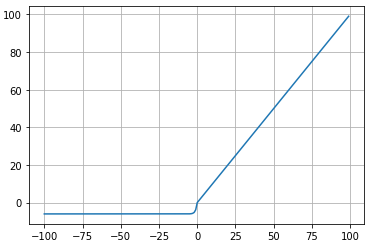
\includegraphics[width=6cm,height=6cm,keepaspectratio]{elu.png}
  \caption{ELU}
  \label{fig:elu}
\end{figure}

\subsubsection{ReLU}
\[
  R(z) = max(0, z)
\]

\par
ReLU funkcija vadinasi: ‘Rectified Linear Unit’. Ši funkcija pasiekia panašų efektyvumą
kaip ir Sigmoid funkcija, tačiau ji reikalauja mačiau skaičiavimo resursų nei sigmoid
ir tanh, nes minėta formulė yra paprastesnė, nei kitos. \cite{salt16}

\begin{figure}[ht]
  \centering
  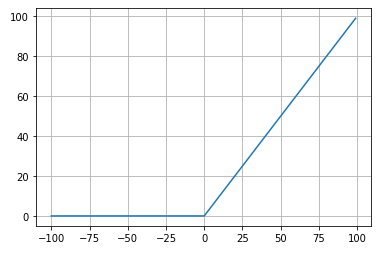
\includegraphics[width=6cm,height=6cm,keepaspectratio]{relu.png}
  \caption{ReLU}
  \label{fig:relu}
\end{figure}

\subsubsection{Sigmoid}
% (https://ml-cheatsheet.readthedocs.io/en/latest/activation_functions.html)
\[
  R(x) = \frac{1}{1 + e^{-x}}
\]

\par
Sigmoid funkcijos parametrai priima realiuosius skaičius ir gražina reikšmę [0; 1].
Šios funkcijos geros savybės yra: tolydus gradientas, prognozuojamas išvesties
diapazonas, netiesiškumas, visur diferencijuojama ir monotoniška. \cite{salt16}

\subsubsection{Softmax}
\[
  softmax(x)_i = \frac{exp(x_i)}{sum_{j=1}^{n}exp(x_j)}
\]

\par
Softmax funkcija priima parametrų skirstinį ir gražina tikimybių skirstinį,
kurio bendra suma yra lygi vienam. \cite{salt16}

\subsubsection{Argumentacija už pasirinktą aktyvacijos funkciją}
% (http://cs231n.github.io/linear-classify/#softmax Stanford university notes)
\par
Šiame darbe bus naudojama Softmax aktyvacijos funkcija. Ši funkcija buvo
pasirinkta, nes galima teigti, jog Softmax bando optimizuoti entropijos
skirtumą tarp tikros reikšmės ir gautos. Entropija tarp tikros reikšmės
‘p’ ir spėjamos ‘q’ yra apskaičiuojama pagal:

\[
H(p, q) = - \sum_{x}p(x) \log q(x)
\]

\par
Pagal entropijos lygtį galima teigti, jog Softmax funkcija
bando optimizuoti entropiją tarp tikros reikšmės ir spėjamos \cite{salt6}.
Tai priveda prie apytiksliai stabilaus gradiento. Jeigu modelis klysta,
jis dėl to gali greičiau pasitaisyti.
\par
Kita priežastis, kodėl yra naudojama Softmax funkcija, yra naudojimui
patogi išvestis. Jeigu norima aptikti kelias klases, kiekvienas išvesties
neuronas išveda klasės tikimybę. Jeigu išvestis yra 0.6, tai tikimybė, kad tai ir
yra ta klasė, yra 60\%. Visų išvesties neuronų išvesties suma yra lygi 1.

\section{Problemos su skaičiaja matematika}
\par
Neuroninius tinklus sudaro paprastai daug sluoksnių ir kiekviename sluoksnyje yra po
daug neuronų. Kiekvienas neuronas yra sudėties funkcija. Funkcija apibrėžia m įvesties
vienetų 'x', su 'w' svoriais. Visi šie neuroniai savo ir kaimyniniuose dviejuose sluoksniuose
yra sujungti su visais kitais neuronais. Pereinant duomenims į kitą sluoksnį yra apskaičiuojamos
visų neuronų reikšmės ir jos perduodamos toliau. Todėl tarp neuroniniame tinkle vyksta
labai daug sudėties operacijų ir yra svarbu, kad neįvyktų jokią skaičiosios matematikos klaida,
kaip reikšmės apvalinimo klaida.

\[
  y_{k} = \gamma \cdot (\sum_{i=1}^{m}w_{ki}x_{i})
\]

Neuroniniai tinklai atlieka daug skaičiavimų, todėl gali atsirasti klaidos su
skaičiaja matematika: gradientinio nuolydžio "užstrigimas", apvalinimo paklaida,
blogas problemos apibrėžimas.

\subsection{"Underflow" ir "overflow"}
% (Ian  Goodfellow Yoshua Bengio, Aaron Courville Deep Learning)
\par
Kai kompiuterinės programos vykdo daug skaičiavimų su
labai dideliais arba mažais skaičiais atsiranda 'underflow' ir 'overflow' problemos
dėl skaičių apvalinimo. ‘Underflow’ problema pasireiškia,
kai funkcijos reikšmė yra labai arti nulio ir ji yra apvalinama į nulį. Kai
kurie algoritmai gali ‘sulūžti’ dėl nulinio parametro (pvz. dalybos iš nulio). Kita
problema yra ‘overflow’. Ji pasireiškia kai gauta reikšmė yra labai didelė ir ji yra
apvalinama į begalybę. \cite{salt7} Vienas iš pavyzdžių kaip pasireiškia 'overflow' problema skaičiavimuose
yra 4 pav. Šiame kode yra paimama didžiausia galima 'Integer' skaičiaus reikšmė ir ji
yra didinama. Taip atsakymas yra apvalinamas į didžiausią galimą reikšmę ir
yra prarandama ta pati reikšmė. Šios dvi problemos yra išspręstos naudojant dviejų bitų statuso registrą
esantį kompiuterio procesoriuje. Vienas bitas yra nustatomas jeigu CPU įvykdo 'overflow', kitas, jeigu
procesorius įvykdo 'underflow'. Modernios programavimo kalbos, kaip Python, pagal šiuos du
bitus gali pasakyti ar įvyko viena iš šitų klaidų.

\begin{figure}[ht]
  \centering
  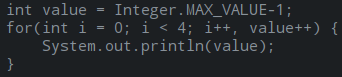
\includegraphics[width=6cm,height=6cm,keepaspectratio]{code1.png}
  \caption{Overflow problema}
  \label{fig:overflowProblem}
\end{figure}

\subsection{Apribotas optimizavimas}
Apribotas optimizavimas yra naudojamas norint optimizuoti funkciją
turint nustatytus kintamuosius.\cite{salt7}
\par
Paprasčiausias šios problemos sprendimas yra didžiausio gradientinio nuolydžio
metodo naudojimas. Pasirinkus pakankamai mažą mokymosi žingsnį ir pradinį tašką, kuris
yra arti tikrosios reikšmės, galima pasiekti kitus neapribotus kintamuosius.

\[
\theta = \theta - \eta \cdot \bigtriangledown_{\theta}J(\theta)
\]

\par
Sudėtingesnis šios problemos sprendimas yra pačios problemos perdarymas. \cite{salt7}

\subsection{Blogas problemos apibrėžimas}

Funkcija yra blogai apibrėžta, jeigu keičiant funkcijos įvestį nedaug, funkcijos reikšmė
pakinta ženkliai daugiau. Funkcija yra laikoma gerai apibrėžta, jeigu keičiant jos įvestį,
jos reikšmė keičiasi proporcingai. Ši problema pasireiškia labiausiai, kai yra
atliekami skaičiavimai su mažais skaičiais. Jeigu įvesties vietoje įvyksta apvalinimo
klaida, funkcijos rezultatas gali grąžinti blogą reikšmę. \cite{salt7}









\section{Optimizavimo algoritmai}
\par
Tinklo siekiamas tikslas yra atliekant kuo mažiau mokymosi iteracijų, pasiekti norimą
išvesties tikslumą. Šiam mokymosi greičiui ir tikslumui pasiekti ir naudojami
optimizavimo algoritmai.

\subsection{Gradientinis nuolydis}
% https://medium.com/@sdoshi579/optimizers-for-training-neural-network-59450d71caf6
% https://towardsdatascience.com/gradient-descent-algorithm-and-its-variants-10f652806a3
Gradientinio nuolydžio algoritmas
Tai yra pati paprasčiausia optimizavimo funkcija.
\[
\theta = \theta - \eta \cdot \bigtriangledown_{\theta}J(\theta)
\]
Pagal algoritmą yra atliekama daug iteracijų. Kiekvienos iteracijos metu yra
apskaičiuojama delta. Ji yra gaunama iš esamos deltos atėmus mokymosi žingsnio konstantos
ir nuostolių funkcijos gradientą parametro delta atžvilgiu. Kadangi žingsnis kurį
atliekame kiekvienos iteracijos metu yra konstanta, jeigu pradinis parinktas taškas
yra toli nuo lokalaus minimumo, tai prireiks daug iteracijų, kol jis bus pasiektas.
Šiuo metodu taip pat kiekviena iteracija yra peržiūrimi visi duomenys, kad nėra
gerai jeigu duomenų yra itin daug. \cite{salt8} Tokiu atveju reikėtų daug atminties. Šis algoritmas nebus naudojamas, nes nėra
atsižvelgta į praeitas iteracijas ir minimumas yra per lėtai pasiekiamas, algoritmas.

\subsection{Poaibio gradientinis nuolydis}
 Šis algoritmas yra panašus į paprastą gradientinį metodą, tačiau yra kelis pakeitimai.
 Kai yra pereinama per visus duomenis, po kiekvieno duomenų elemento peržiūrėjimo,
 yra atnaujinami parametrai. Todėl po kiekvienos iteracijos, turime visų duomenų
 elementų pakeitimų sudėtį. Todėl minimumas yra pasiekiamas statesne trajektorija ir
 nereikalinga turėti daug atminties. Pagrindinis šio metodo trūkumas yra galimas jo
 lėtumas. Pereiti per visus duomenis užtrunka daug laiko ir nevisos duomenų elementų
 iteracijos prie parametrų pakeitimo daug neprisideda. \cite{salt9}

\subsection{Mažo poaibio gradientinis nuolydis}
\[
\theta = \theta - \eta \cdot \bigtriangledown_{\theta}J(\theta;x^{(i:i+n)};y^{(i:i+n)})
\]
\par
Abiejų minėtų algoritmų idėjų kombinacija išvedė mažo poaibio gradientinį metodą.
Šis algoritmas suskirsto duomenis į poaibius, kurių elementų skaičius yra daugiau nei 1.
Dažniausiai poaibių dydis yra pasirenkamas dvejetas pakeltas kokiu nors laipsniu, nes
vaizdo plokštėms tokius poaibius apdoroja geriau. Šis algoritmas yra greitesnis nei poaibio
gradientinis metodas, nes yra išvengiama mažų iteracijų, kurių duomenų elementas mažai
prisideda prie parametrų pakeitimo. Taip pat šio metodo pasiekiamas tikslumas yra didesnis
nei kitų minėtų algoritmų, nes atsitiktinai parenkami poaibiai skiriasi kiekvieno
poaibių paskirstymo metu, taip sudarant daugiau variacijų ir daugiau triukšmo. Kadangi
bendrai yra apdorojama daugiau duomenų variacijų, šis metodas gali pasiekti didesnį
tikslumą. Nors šis metodas gali pasiekti didesnį tikslumą ir yra greitesnis. \cite{salt9}

% gradient descent methods overview
\subsection{Sunkumai taikant gradientinius metodus}
\begin{enumerate}
\item Mokymosi žingsnio nurodymas. Tikslaus sprendimo nurodančio kokį žingsnį parinkti nėra, jis paprastai
yra parenkamas empiriškai stebint konvergavimo greitį ir duomenų kiekį. Jeigu žingsnis yra parenkamas per didelis,
tai optimizavimo funkcija gali diverguoti arba peršokti lokalų minimumą ir nutolti nuo jo, taip praiilginant
procesą. Jeigu žingsnis yra parenkamas per mažas, tada konvergavimo greitis į lokalų minimumą yra labai mažas
ir procesas trunka ilgai. \cite{salt17}
\item Mokymosi žingsnio keitimo trigeris. Kuriant "trigerį" reikia nurodyti arba epochų skaičių arba ribinę nuostolių
funkcijos reikšmę, kada trigeris turi būti aktyvuotas. Po aktyvacijos, trigeris pakeičia mokymosi žingsnio dydį.
Trigerio aktyvacijos laiko nurodymui irgi nėra jokios tikslios taisyklės, tai yra nurodoma empiriškai stebint
mokymosi procesą. Jeigu aktyvacijos laikas yra nurodomas per anksti, mokymosi žingsnis yra sulėtinamas per greitai
ir funkcija pradeda lėčiau diverguoti į minimumą. Jeigu žingsnis yra nurodomas per vėlai, tam tikru momentu
žingsnis gali būti per didelis ir funkcija gali pradėti diverguoti arba peršokti lokalų minimumą ir tolti nuo
minimumo. \cite{salt17}
\item Duomenų rinkinio parinkimas. Jeigu daug duomenų turi tuos pačius požymius, pagal kuriuos tinklas klasifikuoja
rezultatus, visų šių duomenų iteracija nėra būtina, nes jie tinklo svorių pokyčius įtakos labai nežymiai.
Jeigu duomenų, su panašiais požymiais, yra daug, reikia paimti tik dalį jų ir tik tą dalį iteruoti. Jeigu
duomenų, su panašiais požymiais, yra daug, tada tinklo vienos epochos trukmė gali užtrukti ilgiau ir optimizavimo
funkcija lėčiau konverguos į lokalų minimumą. \cite{salt17}
\item Optimizavimo funkcijos "užstrigimas" ties lokaliu minimumu. Optimizavimo funkcijų tinklas yra rasti
globalų minimumo tašką. Tačiau gradientų nuolydžiu pagrįstų algoritmų dažna problema: "užstrigimas" ties
lokaliu minimumu. Gradientas parodo kuria kryptimi funkcija leidžiasi žemyn. Ta kryptimi optimizavimo algoritmas
eina. Pasiekus lokalų minimumą, kai gradientas pradeda didėti, optimizavimo algoritmai baigia darbą. Todėl jeigu yra
blogai parenkamas pirmas taškas, optimizavimo algoritmai "užstrigs" ties lokaliu minimumu. \cite{salt17} Tą išvengti galima prieš algoritmo pradžią
įvertinti funkciją ir parinkti artimus pradinius taškus prie tikrųjų reikšmių. Kitas būdas to išvegti yra naudoti
optimizavimo algoritmus, kurie nesiremia gradientų nuolydžiu. Vienas iš daugelio algoritmų, kuris nesiremia gradientais, yra
banginių judesių pagrįstas optimizavimo algoritmas.
\end{enumerate}
% https://www.sciencedirect.com/science/article/pii/S0965997816300163?casa_token=yI9V7so44bIAAAAA:y_34ijm8Gc4JBSknYd7cH2hqfk2K4h6dpYxZBTR7RGCEa89wP2b5Ohl_FqhK8t8gG9r4qdmGCg
\par
Minėtas banginių optimizavimo algoritmas buvo sukurtas stebint banginių judėjimą, jiems gaudant mažas žuvis. Gaudant žuvis banginiai negali
padaryti status posūkio, todėl gaunant žuvis jie juda aplink žuvis ir po kelių ratų jie pasiekia apskritimo
centrą ir pagauna žuvis. Šis algoritmas yra pagrįstas būtent šiuo judėjimu. \cite{salt10}
%https://www.researchgate.net/publication/328585765_Energy-Efficient_Scheduling_for_a_Job_Shop_Using_an_Improved_Whale_Optimization_Algorithm
\begin{figure}[ht]
  \centering
  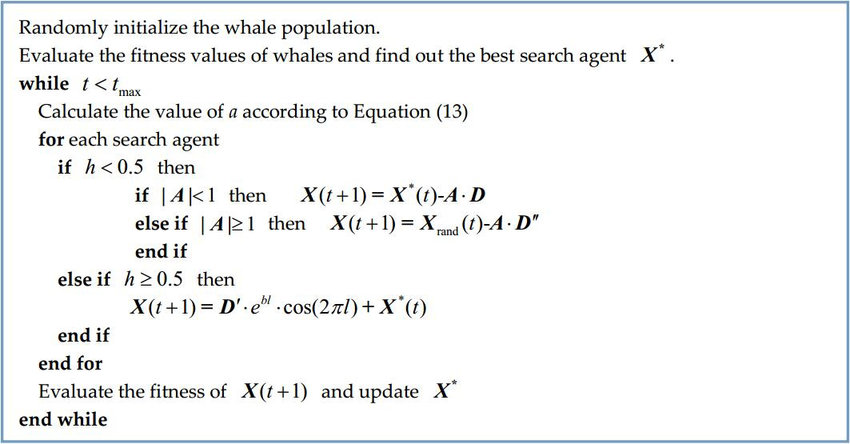
\includegraphics[width=12cm,height=7cm,keepaspectratio]{what_alg.png}
  \caption{Banginių optimizavimo algoritmas \cite{salt10}}
  \label{fig:lygtis1}
\end{figure}







\subsection{Bendros gradientinių metodų problemos}
\par
Gradientinio nuolydžio metodai yra pirmo laipsnio optimizavimo funkcijos, kas
reiškia jog jos naudoja tik pirmo laipsnio išvestines. Kadangi pirma išvestinė rodo
tik funkcijos statumą, bet ne išlenktumą, tai:
\begin{enumerate}
\item Jeigu antra išvestinė yra lygi nuliui, tai funkcija yra tiesinė. Todėl,
mokymosi žingsnis yra lygus alpha. \cite{salt9}
\item Jeigu antra išvestinė yra didesnė už nulį tai funkcijos išlenktumas eina į viršų.
Todėl funkcijos žingsnis yra mažesnis už mokymosi žingsnį ir optimizavimo funkcija gali
diverguoti. \cite{salt9}
\item Jeigu antra išvestinė yra mažesnė už nulį, tai funkcija yra išlenkta į apačią.
Todėl funkcijos žingsnis yra didesnis už mokymosi žingsnį. \cite{salt9}
\end{enumerate}
\par
To pasekoje, optimizavimo funkcijos greitis gali būti lėtas arba ji gali diverguoti.

% TODO PASKAITYTI https://arxiv.org/pdf/1710.08402.pdf

%\subsection{}  Algoritmas kuri naudoja tensorflow

\section{Nuostolių funkcijos}

\subsection{Nuostolių funkcijos pasirinkimas}





% https://towardsdatascience.com/https-medium-com-chayankathuria-regression-why-mean-square-error-a8cad2a1c96f
\par
Nuostolių funkcijos grąžina skirtumą tarp tinklo išvesties ir tikrų reikšmių. Pagal
nuostolių reikšmes yra atitinkamai apskaičiuojami gradientai ir atitinkamai
keičiami tinklo svoriai ir tendenciškumas.

\subsection{Vidutinė kvadratinė paklaida (MSE)}
\[
  Nuostolis = \frac{1}{N} \cdot [\sum(Y_{Gautas}-Y_{Tikras})^{2}]
\]
\par
MSE funkcija sumuoja skirtumų kvadratus ir randa bendrą nuostolių vidurkį.
Ši funkcija yra dažnai numatyta įaviriuose MATLAB ir Python algoritmuose.
Vienintelė neigiama šios funkcijos pusė yra tai, kad jeigu duoti duomenys yra pirmojo
laipsio, tada negalima teigti, kad rezultatai tiesiogiai koreliuoja tarpusavyje,
nes MSE yra antrojo laipsnio funkcija. \cite{salt12}

\subsection{Šaknis iš vidutinės kvadratinės paklaidos (RMSE)}
\[
  Nuostolis = \sqrt{\frac{1}{N} \cdot [\sum (Y_{Gautas}-Y_{Tikras})^{2}]}
\]
RMSE funkcija yra panaši į MSE, tik pridėta šaknies traukimo operacija.
Šaknies traukimas paverčia RMSE pirmojo laipsnio funkcija, todėl ją galima naudoti
su pirmojo laipsnio duomenimis. \cite{salt12}

\subsection{Paklaidų pakelti kvadratu suma}
\[
  Nuostolis = [\sum(Y_{Gautas} - Y_{Tikras})]^{2}
\]

]subsection{Argumentacija už pasirinktą aktyvacijos funkciją}
TODO
% https://www.pyimagesearch.com/2018/11/19/mask-r-cnn-with-opencv/
\section{Neuroninių tinklų modeliai}
\par
Objektų aptikimas nuotraukose, taikant dirbtinius neuroninius tinklus, gali būti kelių
tipų: objektų klasifikacija, objektų lokalizacija, semantinė segmentacija,
objektų segmentacija (instance segmentation).
 \par
 Objektų klasifikacijos tinklas gražiną reikšmę nusakančią ar vaizde yra objektas
 ar jo nėra. Klasifikacijos uždavinį sprenžiant yra pradedama nuo duomenų normalizacijos.
 Visi vaizdai yra padidinami ar sumažinami iki tam tikro dydžio. Galima taip pat pašalinti
 vaizdų RGB kanalą ir padaryti juos bespalviais. Norint padidintį esamą duomenų rinkinį šiame
 darbe buvo naudotas Gauso filtras kiekvienai nuotraukai. Su kiekviena nuotrauka buvo sugeneruotas dar
 5 papildomos su skirtingai Gauso filtro parametrais. Šis metodas taip pat padeda neuroniniam
 tinklui neprisirišti prie tam riktų pikselių reikšmių. Taip pat vaizdus galima pakreipti ir kitaip
 modifikuoti, tačiau plaučių aptikimo tomografiniuose vaizduose uždavinyje, tas nebuvo
 atliktas, nes organai dažniausiai išlaiko savo proporcijas. Po duomenų normalizacijos reikia
 žiūrėti duomenų parametrus ir pagal tai sukonstruoti pirmajį tinklo sluoksnį. Paprastai pirmą sluoksnį
 nusako:
 \[
N_{Pirmas_sluoksnis} = X_{VaizdoPlotis} \cdot Y_{VaizdoAukškis} \cdot N_{SpalvųKanalųSkaičius}
 \]
Sprendžiant plaučių aptikimo kompiuterinės tomografijos nuotraukose uždavinį, buvo naudojamas
RGB kanalų pašalinimas. Taip buvo sumažintas pirmasis tinklo sluoksnis tris kartus ir paleidžiant
sprendimą prireikė mažiau atminties. Paskutinis tinklo sluoksnis priklauso nuo to, kokius mes
rezultatus norime gauti. Jeigu norime pasakyti koks objektas yra nuotraukoje, galima naudoti
tokį išvesties sluoksnio dydį, kiek yra klasių modelyje. Norint taip pat aptikti ir kur
vaizde yra atpažintas objektas tinklo išvesties sluoksnio dydis turi būti:
\[
  N_{Išvesties_sluoksnio_dydis} = C_{KlasiųSkaičius} \cdot 5
\]
Klasių skaičius yra dauginamas iš 5, nes norime gauti pačios klasės tikimybę ir tikėtinas
viršutines ir apatines objekto x ir y reikšmes.Jeigu norime gauti ne tik x ir y reikšmes, bet tikslias
objekto kiekvieno taško koordinates, kad tiksliai žinotume objekto ribas, reikia sudėtingesnio modelio,
kuris vertintų kiekvieno vaizdo pikselio tikimybę, kad jis priklauso tam tikrai klasei.
Šio modelio įvesties sluoksnis lieka toks pat kaip ir kitų, tačiau keičiasi išvesties sluoksnis. Jis tampa
lygus:
\[
N_{IšvestiesSluoknis} = C_{KlasiųSkaičius} \cdot X_{VaizdoPlotis} \cdot Y_{VaizdoAukškis}
\]
Taip galima nusakyti kuriai klasei priklauso kiekvienas pikselis ir nusakyti, kokios yra
kiekvienos klasės ribos vaizde.
\par
Šiame darbe yra naudojamas Tensorflow karkaso Mask RCNN inception modelis, kuris naudoja
objektų segmentavimą. Tinklo modelį ištreniruoti ir nusakyti kur yra tikslios plaučių
ribos nuotraukose, buvo naudojami dvejetainių reikšmių "png" failai. Vienas iš tokių
failų pavyzdžių:

\begin{figure}[ht]
  \centering
  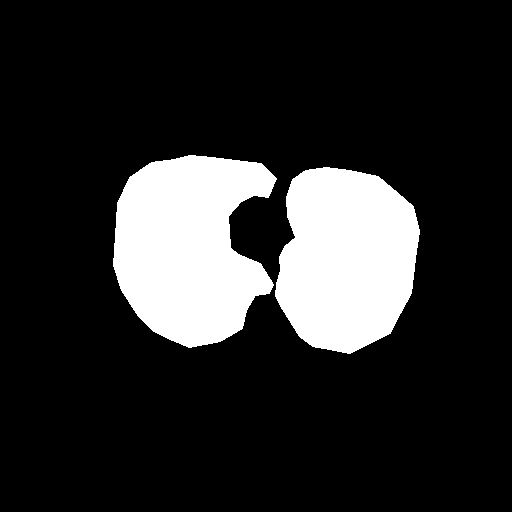
\includegraphics[width=4cm,height=4cm,keepaspectratio]{mask.png}
  \caption{Vaizdo kaukė.}
  \label{fig:kaukė1}
\end{figure}

\par
Šiam uždaviniui tokio tipo failai buvo pasirinkti tam, nes reikia aptikti dvi klases:
plaučiai ir ne plaučiai. Taip su skirtingomis pikselių reikšmėmis yra paduodamos kiekvieno
pikselio klasės. Šie dvejetainiai vaizdų failai buvo gauti apibrėžiant plaučius kiekvienoje
nuotraukoje ir eksportuojant pažymėtus ribinius taškus į "XML" failus. Pagal duotas ribinių
taškų X ir Y koordinates, buvo parašyta programa, kuri automatiškai pagal turimus
duomenis sugeneruoja dvejetainius vaizdų failus.
\par








% https://towardsdatascience.com/computer-vision-instance-segmentation-with-mask-r-cnn-7983502fcad1
\subsection{Mask RCNN inception}
\par
Mask RCNN modelį sudaro dvi dalys: vaizdo regiono pasiūlymo tinklas (Regional proposed network) ir
klasifikavimo modelis. \cite{salt14} Bendras algoritmas:
\begin{enumerate}
\item Nuotrauka yra praleidžiama per konvoliucinį neuroninį tinklą (R-CNN), kuris
sugeneruoja požymių aibę, pagal kurią galima nuspėti, kad tai yra ieškomas objektas
ir kur būtent jis yra vaizde.
\item Vaizdo regiono pasiūlos algoritmas naudoja CNN, kad sugeneruotų regionus vaizde pagal
gautą požymių aibę.
\item Sulyginus gautis regionus gaunamos koordinatės, kurios apibrėžia objektą.
\item Naudojant regresijos modelius objekto apibrėžimas yra tikslinimas, kol gaunami
optimalūs rezultatai.
\item Rezultatai yra persiunčiami į kitą CNN tinklą, kuris sugeneruoja vaizdų kaukes
, atitinkančius klases.
\end{enumerate}
\par
% https://medium.com/@smallfishbigsea/faster-r-cnn-explained-864d4fb7e3f8
Tinklas gauna vaizdo regionus, kurie turi didesnę tikimybę turėti objektą, naudodamas
9 inkarinių apibrėžimų koordinates.
3 inkariniai apibrėžimai yra skirtingų formų. Kiekvienam šiam apibrėžimui yra sukuriami
dar 2 apibrėžimai, kurių formos yra vienodos, tačiau jų dydžiai skiriasi. Šiais 9
inkarais yra pereinama per vaizdą su kiekvienu inkaru ir kiekvienas inkaro apibrėžtas
vaizdas yra analizuojamas: siunčiamas per CNN ir gaunama tikimybė, kad tai yra tam tikra
klasė. Su kiekvienu uždaviniu yra patartina patiems apibrėžti kokios formos turi būti inkarai. \cite{salt15}
Pavyzdžiui jeigu uždavinys yra aptikti plaučius kompiuterinės tomografijos nuotraukose,
inkarai turėtų būti būti didesni į aukštį ir mažesni į plotį ir 3 inkarai iš 9 turi būti
kvadrato formos, nes jeigu analizuojamas plaučių viršus nuotraukose, tai jis yra apvalus,
o ne pailgas.
\par
Turint daug inkarų sudarytų vaizdų, reikia atskirti kurie vaizdai yra fonas, o kurie
yra objektas. Foninių vaizdų negalima traukti į regresijos modelį, o objekto vaizdus reikia.
Šis regresijos modelis yra naudojamas pataisyti inkaro sukurtą vaizdą, kad jis apibrėžtų tik
objektą. \cite{salt15}
\par
Po šių veiksmų vaizdui yra sugeneruojama daug objektų apibrėžimų. Dalis šių apibrėžimų
kertasi tarpusavyje. Apibrėžimai kurie kertasi tarpusavyje yra išsaugomi ir vėliau
toliau analizuojami. \cite{salt15} Kiekvienam kirtimui yra apskaičiuojamas kirtimosi koeficientas:
\[
  K = \frac{N_{PirmasObjektas} \bigcap N_{AntrasObjektas}}{N_{PirmasObjektas} \bigcup N_{AntrasObjektas}}
\]
\par
Jeigu koeficientas yra lygus 1, tai reiškia jog inkarų apibrėžimai sutampa idealiai.
Jeigu koeficientas yra mažesnis už arba lygus 0.5, tada apibrėžimai nėra naudojami.
Jeigu koeficientas yra didesnis už 0.5, sankirta yra išsaugoma tolimesnei analizei.
Atlikus paiešką, kiekvienam atskiram objektui yra parenkama tik sankirta su aukščiausiu
sutapimo koeficientu ir kiti apibrėžimai apie einamąjį objektą yra pašalinami.
Po šių žingsnių yra gaunami apibrėžimai aplink kiekvieną objektą, ir jų yra tik po
vieną. Kiekvienas šis apibrėžimas yra siunčiamas per kitą CNN tinklą, kuris analizuoja
kiekvieno pikselio reikšmę ir nustato tikslias objektų ribas \cite{salt15}.

% https://machinethink.net/blog/mobilenet-v2/
% https://arxiv.org/abs/1512.02325
\subsection{Vieno kadro aptikimas}
\par
Vieno kadro aptikimo (trumpinys SSD) algoritmas objektų aptikimui naudoja tik vieną kadrą.
Objektų aptikui vaizdo įrašuose, objektams aptikti užtenka vieno kadro ir užtenka
duomenis persiųsti per neuroninį tinklą tik vieną kartą. Šis algoritmas
naudoja VGG16 architektūrą kaip pagrindą. Toks pasirinkimas buvo atliktas dėl VGG16
didelės spartos \cite{salt20}. Ieškomos vietos paieška naudojasi inkarų sistema:
yra generuojami langai, vaizdui skanuoti, kurie yra įvairaus dydžio santykių.
Kiekvienam sugeneruotam langui yra skaičiuojama tikimybė, kad tai yra koks objektas
ir atstumą iki tikrosios reikšmės. Sugeneruoto lango nuostoliui apskaičiuoti
yra naudojama L1-Norm. skaičiuojant nuostolius \cite{salt20}. Ši nuostolių funkcija
yra mažiau tiksli negul naujesnė L2-Norm. tačiau ji buvo pasirinkta, nes ji yra nuolaidesnė
kiekvienam pikseliui. T.y. jeigu keli pikseliai neatitinka objekto, o visi kiti atitinka,
tai šie daro mažai įtakos galutiniam tinklo rezultatui.

\subsection{Alternatyvūs objekto paieškos algoritmai}
\par
Minėti tinklų modeliai skiriasi savo neuroninių tinklų struktūra ir ieškomų regionų
paieškos algoritmais. Minėti abu tinklai naudoja skirtingas inkarų paieškos algoritmo
realizacijas. Egzistuoja ir daugiau paieškos būtų. Vienas iš būtų yra slenkančio lango
algoritmas. Šis algoritmas pereina per visas galimas vaizdų kombinacijas. Vietoj
laikantis tam sikro lango dydžio santykio,visi dydžiai yra pasirenkami ir išanalizuojami.
Kadangi šis algoritmas tikrina daugiau sugeneruotų langų kombinacijų, algoritmas veikia labai lėtai.
Buvo sukurtas rašytinių lietuvių kalbos raidžių aptikimo modelis. Jis buvo padarytas iš 3 sluoksnių
ir vienai 1920x1080 pikselių nuotraukai išanalizuoti prireikia vidutiniškai 20 minučių. Tačiau
šį laiką galima sutrumpinti padidinant žingsnio dydį. Pavyzdžiui, padidinus žingsnio dydį vietoj
1 pikselio, naudojant 10-ties pikselių žingsnį, laikas vienai nuotraukai išanalizuoti
vidutiniškai užtrunka apie 6 minutes.

\section{Tyrimas}
\par
Objektų aptikimo kompiuterinės tomografijos nuotraukose uždaviniui sręsti,
buvo naudotas Tensorflow karkasas.
Tyrimas buvo padalintas į kelias dalis: literatūros analizę, modelio
sukūrimą, treniravimą ir jo praktinį pritaikymą programoje.

\subsection{Duomenų paruošimas}
\par
Kompiuterinės tomografijos nuotraukos buvo parsiųstos iš
\enquote{https://www.cancerimagingarchive.net/} puslapio.
Jos kraštinės buvo sužymėtos naudojant \enquote{Make-sense} duomenų žymėjimo programa.
Kiekvienas pažymėtas taškas apibrėžiantis objektus buvo
eksportuotas į JSON failą. Kadangi buvo reikalingi kaukių failai, o buvo turimas,
tik JSON, buvo parašyta kita programa, kuri išanalizuoja JSON failą ir
sukuria kaukes pagal tai. Šiame darbe buvo sužymėtos 50 nuotraukų.
Kiekvienai nuotraukai buvo pritaikytas Gauso filtras su 5 skirtingais
parametrais. Taip buvo gauta 5 kartus daugiau duomenų, negu buvo
sužymėta iš pradžių.
\par
Turint vaizdus ir jų kaukes, reikia šiuos duomenis suspausti į vieną failą.
Tensorflow karkasas treniruojant modelį priima \enquote{.pb} failus mokant modelį.
Duomenų suspaudimui buvo parašyta tam atskira programa kuri naudoja \enquote{object\textunderscore detection}
direktorijoje esančias pagalbines programas.
Galutinis duomenų paruošimo rezultatas: sukurti trys atskiri \enquote{.pb}
failai, kuriuose yra pateikti treniravimo, testavimo ir validavimo duomenys.

\subsection{Modelio sukūrimas ir treniravimas}
\subsubsection{Pasiruošimas}
\par
Prieš naudojamo modelio pasirinkimą apmokymą reikia atlikti keletą
paruošiamųjų žingsnių.
Pirma reikia parsisiųsti Tensorflow karkaso sukurtą modelių rinkinį, kuriame
yra pateikti modeliai ir kiti modeliavimo sprendimai, pagreitinantys darbą.
Šiame rinkinyje yra naudojamos dvi direktorijos: \enquote{object\textunderscore detection} ir \enquote{slim}.
\enquote{object\textunderscore detection} direktorijoje yra pateiktas karkasas, su kuriuo yra lengva
kurti naujus objektų aptikimo modelius ir juos apmokyti. Šis rinkinys turi ir
jau apmokytų modelių pagal COCO duomenų bazę \cite{salt21}. Kitą direktorija \enquote{slim},
yra skirta mokymui ir patikrinimui kaip veikia vaizdų klasifikacijos
modeliai, kaip Inception ir VGG. Parsisiuntus Tensorflow karkaro modelių
rinkinį, reikia parsisiųsti Google Protobuf produktą. Minėtoje \enquote{object\textunderscore detection}
direktorijoje esančiame karkase, yra naudojami \enquote{.proto} failai, kurie turi būti
sukompiliuoti į \enquote{.py} failus. Google Protobuf programa atlieka šį kompiliavimą.

\subsubsection{Kūrimas ir treniravimas}
\par
Paruošta \enquote{object\textunderscore detection} direktorija jau turi paruoštus
modelius, kurie yra ištreniruoti naudojant COCO duomenų bazę.
Kadangi kompiuterinės tomografijos nuotraukose yra reikalingas
didelis tikslumas ir organai yra susispaudę vienas tarp kito taip, kad
sunkiai matosi organų ribos, negalima naudoti duomenų žymėjimui stačiakampius.
Reikia naudoti kaukes kiekvienam objektui sužymėti. Vienas iš modelių, kuris naudoja
kaukes, yra \enquote{mask\textunderscore rcnn\textunderscore inception\textunderscore v2\textunderscore coco}.
\par
Nusistačius koks modelis bus naudojamas, reikia jį sukonfigūruoti.
Naudojamo failo \enquote{pipeline.config} faile reikia nurodyti visus tinklo parametrus.
Vienas iš jų yra klasių skaičius. Šis skaičius nurodo tinklo išeities sluoksnio dydį.
Kadangi šiame darbe yra dirbama tik su plaučių aptikimu, klasių yra tik 1.
Yra nurodomas įvesties vaizdų modifikavimas. Visų jų dydžiai yra pakeičiami į
800x1365 pikelių dydį. Tai reiškia, kad tinklo įvesties sluoksnį sudarys
1.092.000 neuronų. Šis skaičius yra lygus vaizdo dydžio parametrų sandaugai.
Toliau yra nustatomas vaizdo slenkančio branduolio parametrai: žingsnio dydis, kuris yra lygus 2 ir
branduolio dydis, lygus 2. Konfigūraciniame faile taip pat yra nurodoma naudojama
aktyvacijos funkcija, kuri tyrime yra parinkta \enquote{SOFTMAX}.
Tiek žingsnių užtenka modelio apibrėžimui.
\par
Tinklui treniruoti, Tensorflow karkasas \enquote{object\textunderscore detection} direktorijoje
turi paruošęs programa \enquote{legacy/train.py}, kuri tikriną nurodytą
konfiguracinį failą, duotus suspaustas duomenis, modelį ir treniruoja tinklą.
Kas tam tikrą epochų skaičių, tinklo svoriai ir kitos tinklo reikšmės
yra išsaugomos \enquote{.pb} faile, kuris vėliau yra naudojamas, kai norima
užkrauti tinklo reikšmes ir atlikti tolimesnį tinklo treniravimą arba vykdyti
objektų aptikimą vaizduose.

\section{Rezultatai}
\par
Naudojant Tensorflow karkasą ir "mask rcnn inception v2" tinklo modelį, buvo sėkmingai
ištreniruotas tinklas aptikti plaučius su 0.02 nuostoliais.
Tikslaus tikslumo procentais negalima nusakyti, nes tai yra ne objektų klasifikavimo,
bet aptikimo uždavinys.
Treniravimas užtruko apie 20 minučių,
naudojant Google Colab GPU. Užteko 31240 epochų apmokyti plaučių aptikimą.
Treniravimui buvo sužymėtos 50 nuotraukų. Naudojant žymėjimo programą, buvo sukurti kaukių
failai, kurie tiksliai apibrėžia plaučių ribas. Naudojant įvairias modifikacijas:
gauso filtras pritaikytais 5-iomis skirtingomis tikimybėmis, buvo gautos 298 nuotraukos.
Kadangi nuostoliai nuo ~2500 epochos stabiliai laikėsi ir nustojo mažėti, reiškia norint
pasiekti dar didesnį tinklo tikslumą, reikia sužymėti daugiau duomenų.
Galutinis programos rezultatas pavaizduotas pav. programa. Programos kodas naudoti
duomenys yra patalpinti internete, adresas pateiktas priejų skiltyje.
Šis darbas įrodo, jog pasiekti aukštą
objektų aptikimą kompiuterinės tomografijos nuotraukose, nereikia turėti daug duomenų ir daug
resursų. Tai įmanoma padaryti ir naudojant Google Cloud platformą, kuri suteikia
nemokamą prieigą prie GPU resursų.


\begin{figure}[ht]
  \centering
  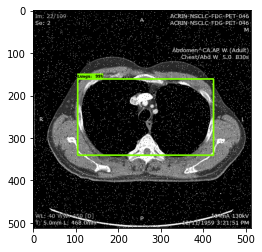
\includegraphics[width=4cm,height=4cm,keepaspectratio]{result1.png}
  \caption{Programa.}
  \label{fig:kaukė1}
\end{figure}

\sectionnonum{Išvados}
% Išvadose ir pasiūlymuose, nekartojant atskirų dalių apibendrinimų,
% suformuluojamos svarbiausios darbo išvados, rekomendacijos bei pasiūlymai.
\par
Pasitelkiant Tensorflow karkasą ir neuroninių tinklų pagalba galima sukurti programą,
kuri aptinka objektus kompiuterinės tomografijos nuotraukose. Apmokyti tinklą
nereikia daug duomenų, vienai klasei apmokyti užtenka 50-ties nuotraukų.
Jos yra modifikuojamos: pridedamas įvairių stiprumo triukšmas. Po maždaug 3000 epochų,
tinklas aptiko plaučius su 0.02 nuostoliais naudojant MSE nuostolių funkciją.


\printbibliography[heading=bibintoc] % Literatūros šaltiniai aprašomi
% bibliografija.bib faile. Šaltinių sąraše nurodoma panaudota literatūra,
% kitokie šaltiniai. Abėcėlės tvarka išdėstoma tik darbe panaudotų (cituotų,
% perfrazuotų ar bent paminėtų) mokslo leidinių, kitokių publikacijų
% bibliografiniai aprašai (šiuo punktu pasirūpina LaTeX). Aprašai pateikiami
% netransliteruoti.

\end{document}
